%%%%%%%%%%%%%%%%%%%%%%%%%%%%%%%%%%%%%%%%%%%%%%%%%%%%%%%
% Please note that whilst this template provides a 
% preview of the typeset manuscript for submission, it 
% will not necessarily be the final publication layout.
%
% letterpaper/a4paper: US/UK paper size toggle
% num-refs/alpha-refs: numeric/author-year citation and bibliography toggle


%\documentclass[letterpaper]{oup-contemporary}
\documentclass[a4paper,num-refs]{oup-contemporary}



%%% Journal toggle; only specific options recognised.
%%% (Only "gigascience" and "general" are implemented now. Support for other journals is planned.)%
%\journal{Test}
\jname{Università degli studi Roma Tor Vergata}
\jlogo{}

\usepackage{graphicx}
\usepackage{siunitx}
\usepackage{import}
%\numberwithin{equation}{section}% numera eq come #section.#formula
%

\usepackage{enumitem}
%
\usepackage{amsmath}
\usepackage{amsthm}
\usepackage{amssymb}
\usepackage{stmaryrd}
%
\usepackage{caption}
\usepackage{subcaption}

\usepackage{wasysym}
\usepackage{cancel}
\usepackage{textcomp}
\usepackage{cleveref}
\newcommand{\crefrangeconjunction}{ {a}\nobreakspace}
\crefname{table}{tab}{tabs}
\crefname{section}{sez}{sezioni}
\renewcommand{\figurename}{Fig.}
\captionsetup[figure]{name={Fig.}}
\captionsetup[sub]{font=scriptsize,labelfont={rm,sf},labelformat=simple}
\newcommand\crefpairconjunction{ e }
\renewcommand\thesubfigure{(\roman{subfigure})}


\crefformat{section}{\S#2#1#3} % see manual of cleveref, section 8.2.1
\crefformat{subsection}{\S#2#1#3}
\crefformat{subsubsection}{\S#2#1#3}
\usepackage{lipsum}  
\usepackage{listings}
\definecolor{codegreen}{rgb}{0,0.6,0}
\definecolor{codegray}{rgb}{0.5,0.5,0.5}
\definecolor{codestring}{rgb}{0.4,0.4,0.4}
\definecolor{backcolour}{rgb}{0.96,0.96,0.96}
\definecolor{bbcolour}{rgb}{0.01,0.03,0.35}
\definecolor{indexcolour}{rgb}{0,0.4,0.4}
\lstdefinestyle{mystyle}{
	backgroundcolor=\color{backcolour},   
	commentstyle=\color{codegreen},
	classoffset=1,
	keywordstyle=\color{bbcolour},
	numberstyle=\tiny\color{codegray},
	stringstyle=\color{codestring},
	basicstyle=\ttfamily\small,
	breakatwhitespace=false,  
	breaklines=true,                 
	captionpos=b,                    
	keepspaces=false,                 
	numbers=left,                    
	numbersep=3pt,                  
	showspaces=false,                
	showstringspaces=false,
	showtabs=false,                  
	tabsize=2
}
\lstset{texcl=false, mathescape=true,style=mystyle}
\lstset{emph={%  
		i, j,X,n,Y,alpha_,axialLoad_,trasLoad_%
	},emphstyle={\color{indexcolour}}%
}%

\usepackage[euler]{textgreek}


\usepackage{tikz}
\usetikzlibrary{shapes.geometric, arrows}
\tikzstyle{startstop} = [rectangle, rounded corners, minimum width=3cm, minimum height=1cm,text centered, draw=black, fill=backcolour]
\tikzstyle{startstop2} = [rectangle, rounded corners, minimum width=3cm, minimum height=2cm,text centered, draw=black, fill=backcolour]
\tikzstyle{io} = [trapezium, trapezium left angle=70, trapezium right angle=110, minimum width=2cm, minimum height=1cm, text centered,text width=2cm, draw=black, fill=backcolour]
\tikzstyle{io2} = [trapezium, trapezium left angle=70, trapezium right angle=110, minimum width=2cm, minimum height=1cm, text centered, draw=black, fill=backcolour]
\tikzstyle{process} = [rectangle, minimum width=3cm, minimum height=1cm, text centered,text width=4cm, draw=black, fill=backcolour]
\tikzstyle{decision} = [diamond, minimum width=2cm, minimum height=1cm, text centered, draw=black, fill=backcolour]
\tikzstyle{arrow} = [thick,->,>=stealth]
\tikzstyle{process2} = [rectangle, minimum width=2cm, text width=2cm,minimum height=1cm, text centered, draw=black, fill=backcolour]
\tikzstyle{process3} = [rectangle, minimum width=2cm,text width=2cm, minimum height=1cm, text centered, draw=black, fill=backcolour]


\definecolor{myred}{rgb}{0.545, 0.172, 0.031}
\usepackage[T1]{fontenc}
\usepackage[utf8]{inputenc}
\usepackage[italian, english]{babel}
\graphicspath{{figures/}} %Setting the graphicspath
\makeatletter
\providecommand*{\input@path}{}
\edef\input@path{{figures/}{}\input@path}% prepend
\makeatother
\usepackage{fancyhdr}

%%% Flushend: You can add this package to automatically balance the final page, but if things go awry (e.g. section contents appearing out-of-order or entire blocks or paragraphs are coloured), remove it!
% \usepackage{flushend}

\title{Risposta strutturale di elementi strutturali laminati}

%%% Use the \authfn to add symbols for additional footnotes, if any. 1 is reserved for correspondence emails; then continuing with 2 etc for contributions.
\author{Mastrofini Alessandro}

%\affil[1]{First Institution}
%\affil[2]{Second Institution}

%%% Author Notes
\authnote{alessandro.mastrofini@alumni.uniroma2.eu}
%\authnote{\authfn{2}Contributed equally.}

%%% Paper category
\papercat{Meccanica Computazionale dei Tessuti e Biomateriali}

%%% "Short" author for running page header
\runningauthor{}

%%% Should only be set by an editor%
%\jvolume{00}
\jyear{2021}

\begin{document}

\begin{frontmatter}
\maketitle
\begin{abstract}

Nella presente analisi sono state condotte diverse campagne di simulazione per analizzare la risposta strutturale di un composito laminato CF/PEEK che mostra grandi potenzialità di applicazione nel campo biomedicale. 

 \textbf{Background}, in un composito laminato il comportamento strutturale dipende dalla disposizione dei singoli strati, in queste analisi viene indagato come i differenti layouts influenzano la risposta di alcuni elementi strutturali;
 
  \textbf{Results}, differenti campagne di simulazione mostrano la variazione della rigidezza e delle condizioni di accoppiamento tra le condizioni di carico e la risposta strutturale al variare del layout e dell'angolo di fibratura della lamina;
  
   \textbf{Conclusions}, le risposte strutturali sono molto variabili, da comportamenti più semplici da predire a risposte più complesse. Un'analisi che tiene conto del layout dell'intero laminato, a partire dalla composizione del singolo layer, permette di avere risultati precisi per comprendere il comportamento strutturale.;
   

\end{abstract}

\begin{keywords}
laminates; CF/PEEK; laminates composites mechanics; 
\end{keywords}
\end{frontmatter}



\section{Introduzione}

Lo scopo della seguente analisi è quello di indagare il comportamento di differenti layouts di un composito laminato.

Viene analizzato un composito laminato CF/PEEK, ovvero un composito a matrice polimerica termoplastica rinforzata con fibre di carbonio che mostra grandi potenzialità per le applicazioni biomedicali. Vengono considerati due elementi strutturali fondamentali, un cilindro e una piastra, e viene studiato come la variazione del layout porta ad una differente risposta meccanica.  

Viene fatto anche uno studio approfondito andando ad analizzare la distribuzione delle tensioni a livello dei singoli strati. 

La conoscenza e la possibilità di prevedere il comportamento strutturale a partire dalla disposizione dei layers risulta fondamentale sia per la corretta simulazione che per la produzione di dispositivi ed oggetti con compositi laminati. 


\section{Laminati CF/PEEK} 

I recenti progressi nei materiali compositi, in particolare a matrice PEEK, ovvero una matrice polimerica di poli-eter-eter chetone, hanno ampliato fortemente gli scenari applicativi facendo rientrare questi materiali nella classe dei tecnopolimeri. Questo polimero, viste le sue proprietà, si pone tra i polimeri più importanti in ambito ingegneristico. Ha delle proprietà eccellenti quali un'alta resistenza meccanica, ottima stabilità termica, resistenza chimica e un comportamento stabile anche in ambienti chimicamente ostili. Presenta anche una natura anticorrosiva e una buona resisitenza alla degradazione, proprietà che lo rendono ottimo per le applicazioni in campo biomedicale. 

In tali applicazioni sono state migliorate anche alcune proprietà superficiali combinando il PEEK con particelle bioattive come l'idrossiapatite. Questo ha permesso di far fronte ad alcune problematiche come la limitata efficacia nel far aderire cellule e nell'integrazione con l'osso.  Chiaramente l'integrazione di fibre di rinforzo ne ha permesso anche il miglioramento delle proprietà meccaniche. 

Uno dei rinforzi più importanti è quello a fibre di carbonio uniderizionali. Indicato come CF/PEEK è stato introdotto intorno al 1980 e negli ultimi anni si è mostrato essere un ottimo biomateriale con grandi potenzialità di applicazione negli impianti biomedicali \citep{Verma}.    
PEEK generici trovano grandi applicazioni sia in impianti personalizzati realizzati con stampa 2D sia nell'ortodonsistica. Inoltre, il CF/PEEK trova grandi applicazioni in ortopedia.  È bene sottolineare anche che il CF/PEEK a fibre continue mostra proprietà meccaniche migliori di PEEK generici o rinforzati a fibre corte ma richiede metodi di produzione più avanzati.

Tipicamente in ortopedia sono utilizzati impianti metallici con una rigidezza di circa un ordine di grandezza più elevato di quello dell'osso fisiologico e questo può portare a problematiche legate al riassorbimento osseo. Inoltre, possono esserci problematiche legate all'imaging diagnostico CT o a raggi X \citep{Rohner}. 
L'utilizzo di materiali compositi può fornire diversi vantaggi quali la presenza di proprietà anisotrope, radiotrasparenza, elevata resistenza a fatica ed un elevato rapporto resistenza/peso.  Attualmente sono ancora pochi i compositi laminati effettivamente usati nelle applicazioni ortopediche. Un esempio di tale materiale è un PEEK rinforzato a fibra di carbonio continua, noto come PEEK-OPTIMA\textsuperscript{TM}  Ultra-Reinforced, ed è stato approvato per l'impianto anche negli esseri umani dalla Food and Drug Administration americana \citep{PEEKOPTIMA}.

La campagna di simulazioni seguente fa riferimento ad un composito laminato con strati di CF/PEEK con frazione volumetrica di fibre del 62 \% e ne considera diversi layouts laminati analizzando le performance meccaniche e la risposta strutturale.  



\section{Background}

\begin{figure*}[bt!]
	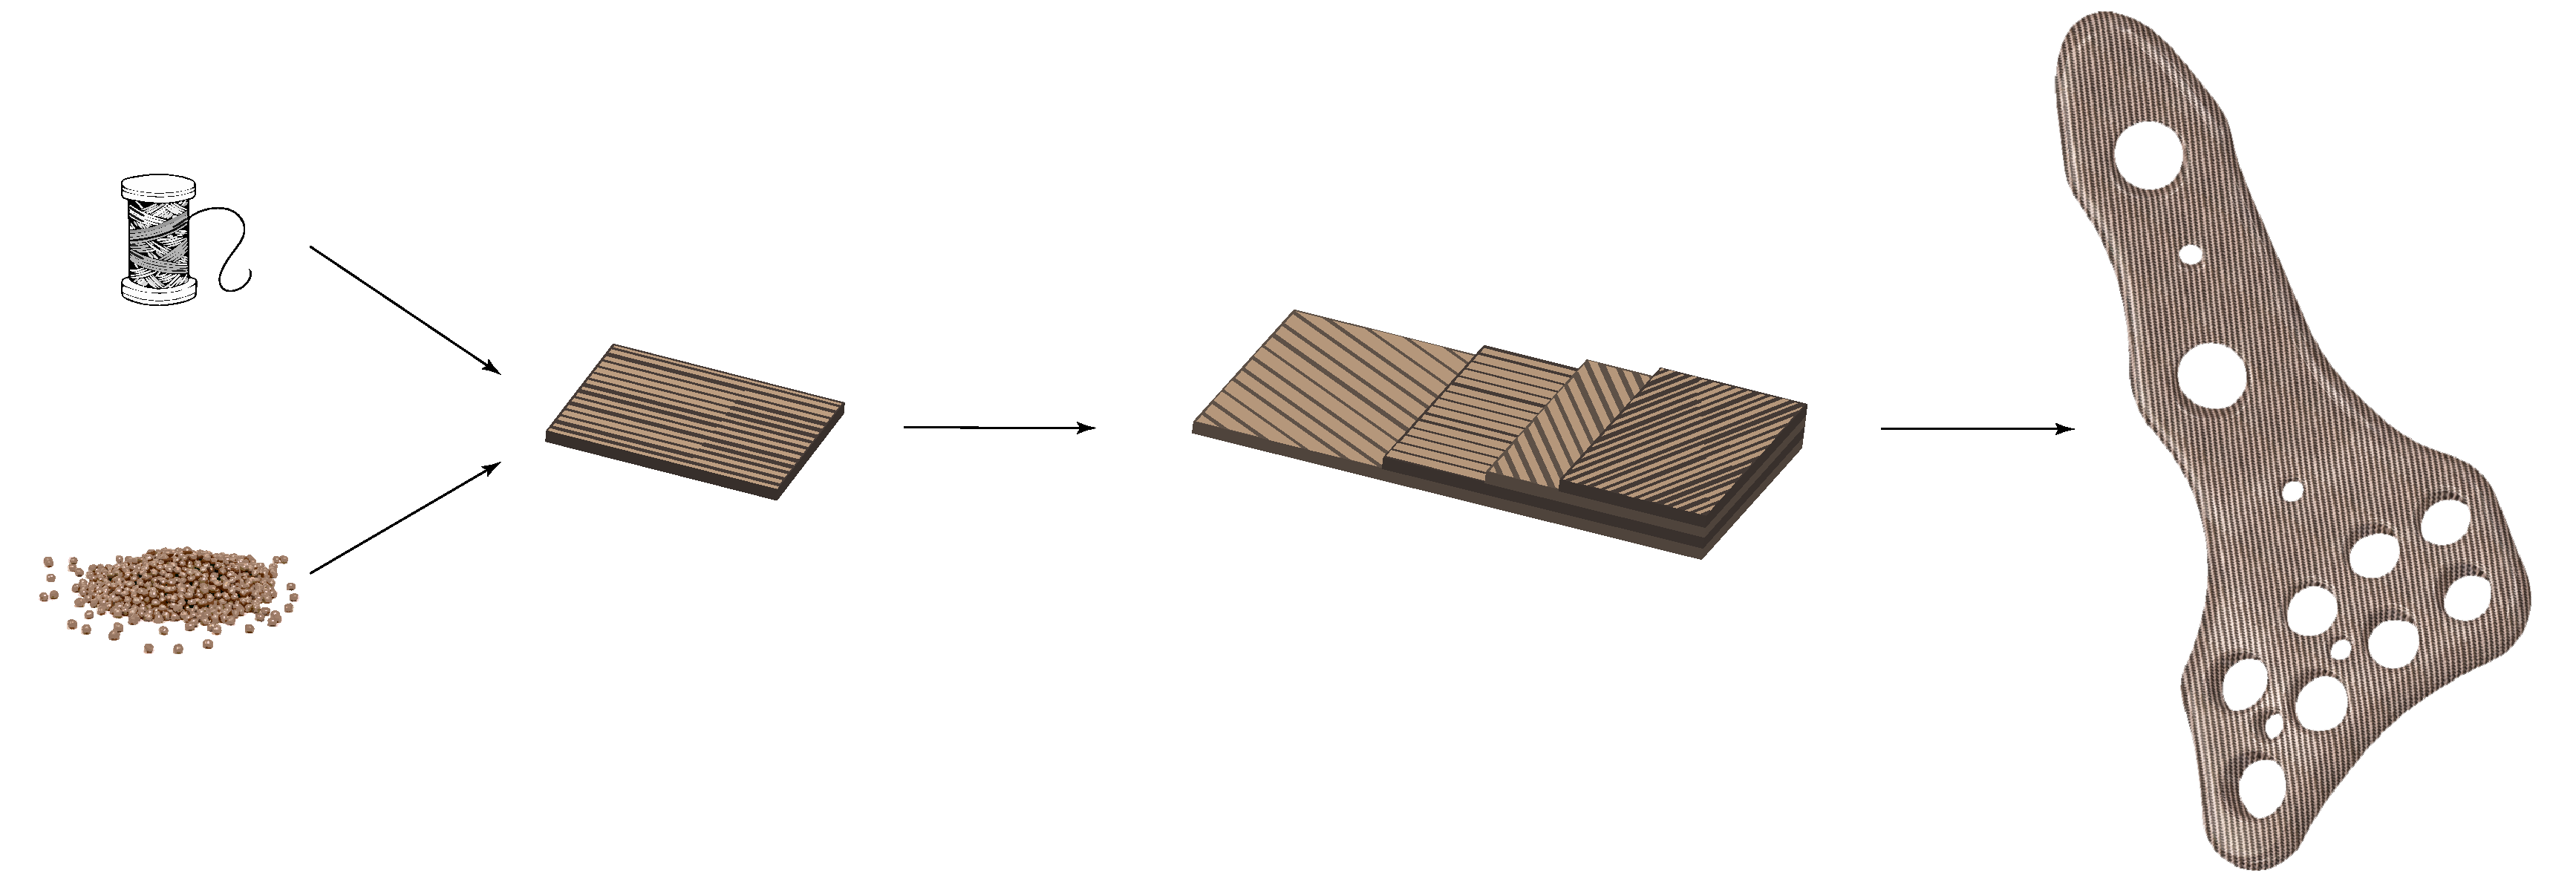
\includegraphics[width=\textwidth]{laminate_figures.pdf}
	\caption{Il comportamento meccanico della struttura finale alla macroscala è fortemente influenzato dai singoli componenti in cascata. Da sinistra: fibre continue di carbonio e pellet di polimero; singola lamina; piastra multi layer; placca ortopedica di fissaggio per il radio distale \citep{MUGNAI2018877,DISTAL}.}
\label{fig:laminates_general}
\end{figure*}

I compositi moderni si basano sull'utilizzo di una fase di rinforzo, tipicamente sotto forma di fibra, immersa in una matrice. Solitamente si utilizza una matrice polimerica e come fibre di rinforzo si possono usare vetro, carbonio, aramide ed altri. Esistono diversi metodi per disporre le fibre e la loro distribuzione influenza il comportamento globale. 

Mettendo insieme più strati di materiale composito si ottiene un pacchetto che prende il nome di composito laminato.

Il problema può essere diviso su tre scale di grandezza differenti: il comportamento della struttura finale (macroscala) che dipende dal laminato che a sua volta è influenzato dalle singole lamine (mesoscala). A loro volta il comportamento è determinato dai singoli costituenti e dalla loro composizione (microscala). Una rappresentazione schematica è data in \cref{fig:laminates_general}.


\subsection{Regola delle miscele}

La singola lamina è composta da una matrice e dalle fibre di rinforzo con una frazione volumetrica precisa. Il primo passo è quello di omogenizzare le proprietà materiali del singolo strato. Consideriamo una fibratura tale da garantire una simmetria trasversalmente isotropa e con direzione di isotropia l'asse della fibra. 

Per arrivare alle proprietà omogenizzate del singolo layer è possibile applicare la regola delle miscele \citep{Kollar:1}.

Considerando un volume globale del composito dato dalla somma del volume della matrice e di quello del rinforzo e assumendo un'adesione perfetta tra i due è possibile calcolare analiticamente i moduli risultanti. Valgono le frazioni volumetriche:

\begin{equation}
v_m+f_f=1   
\end{equation}

Ed è possibile esprime le proprietà materiali risultanti in funzione della frazione volumetrica di fibre ($f_f$) e delle proprietà materiali dei singoli costituenti, come espresso nelle \cref{eq:E1,eq:E2,eq:G12,eq:nu12,eq:nu23,}. 

\begin{equation}
E_1=f_f E_f+\left(1-f_f\right)E_m
\label{eq:E1}
\end{equation}

\begin{equation}
{E_2}=E_3=\left({1-f_f\over E_m}+{f_f\over E_f}\right)^{-1}
\label{eq:E2}
\end{equation}

\begin{equation}
G_{12}=\left(\frac{v_{m}}{G_{m}}+\frac{v_{f}}{G_{f}}\right)^{-1}
\label{eq:G12}
\end{equation}

\begin{equation}
\nu_{12}=v_{f} \nu_{f}+v_{m} \nu_{m}
	\label{eq:nu12}
\end{equation}

\begin{equation}
\nu_{23}=\frac{E_{2}}{2 G_{23}}-1=\frac{E_{2}}{2 G_{12}}-1
	\label{eq:nu23}
\end{equation}

È possibile considerare una matrice di cedevolezza del tipo in \cref{eq:SS}

\begin{equation}
\begin{bmatrix}
	\frac{1}{E_{1}} & -\frac{\nu_{21}}{E_{2}} & -\frac{\nu_{31}}{E_{3}} & 0 & 0 & 0 \\
	-\frac{\nu_{12}}{E_{1}} & \frac{1}{E_{2}} & -\frac{\nu_{32}}{E_{3}} & 0 & 0 & 0 \\
	-\frac{\nu_{13}}{E_{1}} & -\frac{\nu_{23}}{E_{2}} & \frac{1}{E_{3}} & 0 & 0 & 0 \\
	0 & 0 & 0 & \frac{1}{G_{23}} & 0 & 0 \\
	0 & 0 & 0 & 0 & \frac{1}{G_{13}} & 0 \\
	0 & 0 & 0 & 0 & 0 & \frac{1}{G_{12}}
\end{bmatrix}
\label{eq:SS}
\end{equation}

\begin{figure}
\def\svgwidth{\linewidth}
  \input{miture_rule_result_tex.pdf_tex}
	\caption{Andamento dei moduli tipo Young $E_1$ ed $E_2$ e del modulo di taglio $G_{12}$ al variare di $f_f\in \left[0.3;0.9\right]$.}
		\label{fig:mixtureRule} 
\end{figure}

In particolare, è possibile osservare l'andamento dei moduli tipo Young nella \cref{fig:mixtureRule}. È evidente l'andamento lineare di $E_1$. Tutti i moduli aumentano all'aumentare della $f_f$ in quanto aumenta il contributo delle fibre di carbonio che presentano moduli più alti del PEEK. 

L'analisi seguente considera una $f_f$ fissata al 62\%. 




\subsection{Teoria dei laminati sottili }

Dopo aver omogenizzato il singolo layer si ricorre alla teoria dei laminati sottili \citep{SOTTILI} trattando il singolo layer come una lastra sottile omogenea. Ogni lamina è soggetta ad uno stato piano di tensione e la matrice di rigidezza nel singolo strato può essere espressa rispetto un sistema di riferimento globale. 
\begin{equation}
[\bar{Q}]=\left[T_{\sigma}\right]^{-1}[Q]\left[T_{\epsilon}\right]
\label{eq:rotazione}
\end{equation}

Considerando le deformazioni nel piano della superficie media e la curvatura della superficie media si arriva alle leggi costitutive generalizzate, \cref{eq:constitutive}.

\begin{equation}
	\small{
\left[\begin{matrix}
	N_{x} \\
	N_{y} \\
	N_{x y} \\
	M_{x} \\
	M_{y} \\
	M_{x y}
\end{matrix}\right]=\left[\begin{matrix}
	A_{11} & A_{12} & A_{16} & B_{11} & B_{12} & B_{16} \\
	A_{21} & A_{22} & A_{26} & B_{21} & B_{22} & B_{26} \\
	A_{61} & A_{62} & A_{66} & B_{61} & B_{62} & B_{66} \\
 B_{11} & B_{12} & B_{16} & D_{11} & D_{12} & D_{16} \\
	B_{21} & B_{22} & B_{26} & D_{21} & D_{22} & D_{26} \\
	B_{61} & B_{62} & B_{66} & D_{61} & D_{62} & D_{66}
\end{matrix}\right]\left[\begin{matrix}
	\varepsilon_{x}^{o} \\
	\varepsilon_{y}^{o} \\
	\gamma_{x y}^{o} \\
	\kappa_{x}^{o} \\
	\kappa_{y}^{o} \\
	\kappa_{x y}^{o}
\end{matrix}\right]}
\label{eq:constitutive}
\end{equation}

Dove i tre blocchi della matrice hanno un significato preciso. Il blocco $A$, \cref{eq:A},descrive la rigidezza mebranale della singola lamina. Il blocco $B$, \cref{eq:B}, lega l'accoppiamento tra gli effetti membranali e flessionali. Il blocco $D$, \cref{eq:D}, rappresenta la rigidezza flessionale del laminato.


\begin{equation}
A_{i j}=\sum_{k=1}^{N} \bar{Q}_{i j}^{k}\left(z_{k}-z_{k-1}\right)
\label{eq:A}
\end{equation}

\begin{equation}
B_{i j}=\frac{1}{2} \sum_{k=1}^{N} \bar{Q}_{i j}^{k}\left(z_{k}^{2}-z_{k-1}^{2}\right)
\label{eq:B}
\end{equation}

\begin{equation}
D_{i j}=\frac{1}{3} \sum_{k=1}^{N} \bar{Q}_{i j}^{k}\left(z_{k}^{3}-z_{k-1}^{3}\right)
\label{eq:D}
\end{equation}


Tale descrizione permetterà di prevedere gli accoppiamenti e il comportamento strutturale a partire dalla struttura dei tre blocchi. 


\subsection{Proprietà dei costituenti}

\begin{table}[bt!]
	\centering
	\captionsetup{justification=centering}
	
	\caption{Parametri materiali \citep{Gallagher}}

	\begin{tabular}{ m{0.4\linewidth} m{0.4\linewidth}  }
		\toprule
		CF & PEEK\\
		\midrule
		$E_{f}=236$ GPa & $E_{m}=$ 4 GPa   \\
		$\nu_{f}= 0.2$ & $\nu_{m}= 0.36$ \\
		$G_f=27.6 $ GPa & $G_m=1.47$ GPa \\
		\bottomrule
	\end{tabular}
	\label{tab:parametri}
\end{table}

Partendo dal singolo layer, viene considerata una matrice polimerica PEEK che presenta un modulo elastico relativamente basso, di 4 GPa con coefficiente di Poisson $\nu =0.36$. La matrice  viene rinforzata con fibre di carbonio che invece presentano un'elevata rigidezza, modulo elastico di 236 GPa e un coefficiente di Poisson di 0.2. Maggiori informazioni in \cref{tab:parametri}. 

I risultati della regola delle miscele considerando una frazione volumetrica di fibre del 62\% sono riportati in \cref{tab:miscele}.  A partire da questi risultati numerici, viene calcolata la matrice di rigidezza del singolo layer. 

Si procede poi nel considerare diverse configurazioni di laminato. Ogni singolo strato viene considerato con le fibre allineate lungo una direzione principale, ad eccezione dei layer $\pm 45^f$ che vengono considerati come un intreccio di fibre. I singoli layer sono poi ruotati rispetto un riferimento globale e messi insieme a formare il laminato composito. Quindi è possibile calcolare il legame costitutivo generalizzato del laminato.

\begin{table}[h!]
	\centering	
	\begin{tabular}{ m{0.4\linewidth} m{0.4\linewidth}  }
		\toprule
		$ff$  & 0.62 \\
		$E_{1}$  & 147.96 GPa  \\
		$E_{2}$  & 10.83 GPa  \\
		$\nu_{12}$ & $0.26$ \\
		$G_{12}$ & 4.24 GPa \\
		\bottomrule
	\end{tabular}
	\captionsetup{justification=centering}
	\caption{Risultati applicando la regola delle miscele}
	\label{tab:miscele}
\end{table}

\section{Layout del laminato}

\begin{figure*}[bt!]
	\centering\captionsetup[subfigure]{justification=centering}
	
	\begin{subfigure}[c]{0.24\textwidth}
		\centering
	\def\svgwidth{\textwidth}
\input{struct1_tex.pdf_tex}
		\caption{$[\alpha /-\alpha / 30 /-30 / 0_{2}]_{\mathrm{s}}$ }
		
	\end{subfigure}
	\hfill
	\begin{subfigure}[c]{0.24\textwidth}
		\centering 
		\def\svgwidth{\textwidth}
\input{struct2_tex.pdf_tex}
		\caption{$[-45 / 45 /-45 / 45]$}
		
	\end{subfigure}
	\hfill
	\begin{subfigure}[c]{0.24\textwidth}
		\centering
		\def\svgwidth{\textwidth}
\input{struct3_tex.pdf_tex}
		\caption{$[\pm 45^{f} / \pm 45^{f}]$}
		
	\end{subfigure}
	\hfill
	\begin{subfigure}[c]{0.24\textwidth}
		\centering
		\def\svgwidth{\textwidth}
		\input{struct4_tex.pdf_tex}
		\caption{$[-30 /-45 /-30 /-45]$}
		
	\end{subfigure}
	\hfill
	\caption{Differenti layout di laminato considerati nell'analisi}
	\label{fig:laminates}
\end{figure*}

Le variazioni del layout del laminato sono infinite, è possibile variare il numero di strati e l'angolo di fibratura. Nella seguente analisi vengono affrontati 4 casi differenti:

\begin{enumerate}[label=(\alph*)]
	\item $\left[\alpha /-\alpha / 30 /-30 / 0_{2}\right]_{\mathrm{s}}$ con $\alpha\in\left[0^\circ;90^\circ\right]$
	\item $\left[-45 / 45 /-45 / 45\right]$
	\item $\left[\pm 45^{f} / \pm 45^{f}\right]$
	\item $\left[-30 /-45 /-30 /-45\right]$
\end{enumerate}

Un'illustrazione rappresentativa dei differenti layout è presente in \cref{fig:laminates}.

Vengono considerati due elementi strutturali differenti:
\begin{itemize}
\item Elemento tipo piastra
\item Elemento tipo cilindro
\end{itemize}

\begin{figure*}[bt!]
	\centering
	\begin{subfigure}[t]{0.24\textwidth}
		\centering
\def\svgwidth{\linewidth}
\input{plate_tex.pdf_tex}
	 				\caption{Elemento tipo piastra}
		\label{fig:y equals x}
	\end{subfigure}
	\hfill
	\begin{subfigure}[t]{0.24\textwidth}
		\centering
		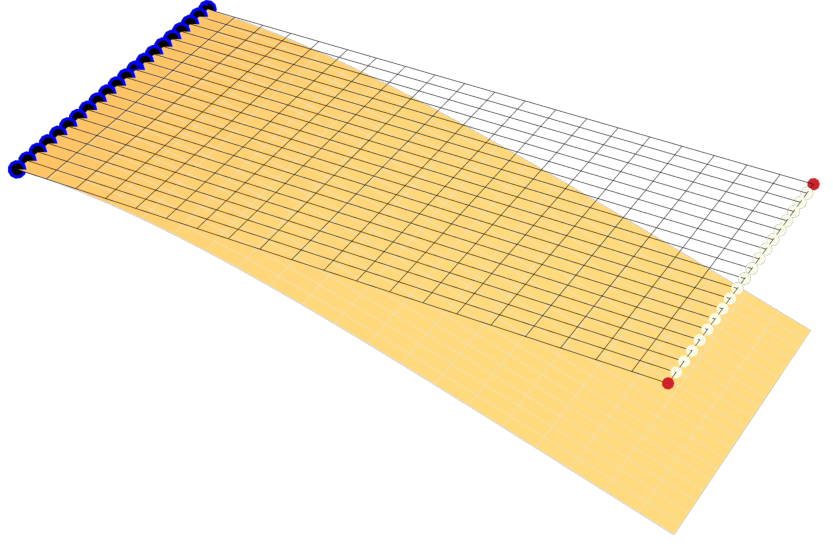
\includegraphics[width=\textwidth]{/first_test/alpha=40.pdf}
		\caption{Elemento tipo piastra deformato \\(caso \cref{sec:plate_A}  con $\alpha=40^\circ$ )}
		\label{fig:five over x}
	\end{subfigure}
	\hfill
	\begin{subfigure}[t]{0.24\textwidth}
		\centering
\def\svgwidth{\linewidth}
\input{cyl_tex.pdf_tex}
\caption{Elemento tipo cilindro}
		\label{fig:three sin x}
	\end{subfigure}
	\hfill
	\begin{subfigure}[t]{0.24\textwidth}
	\centering
 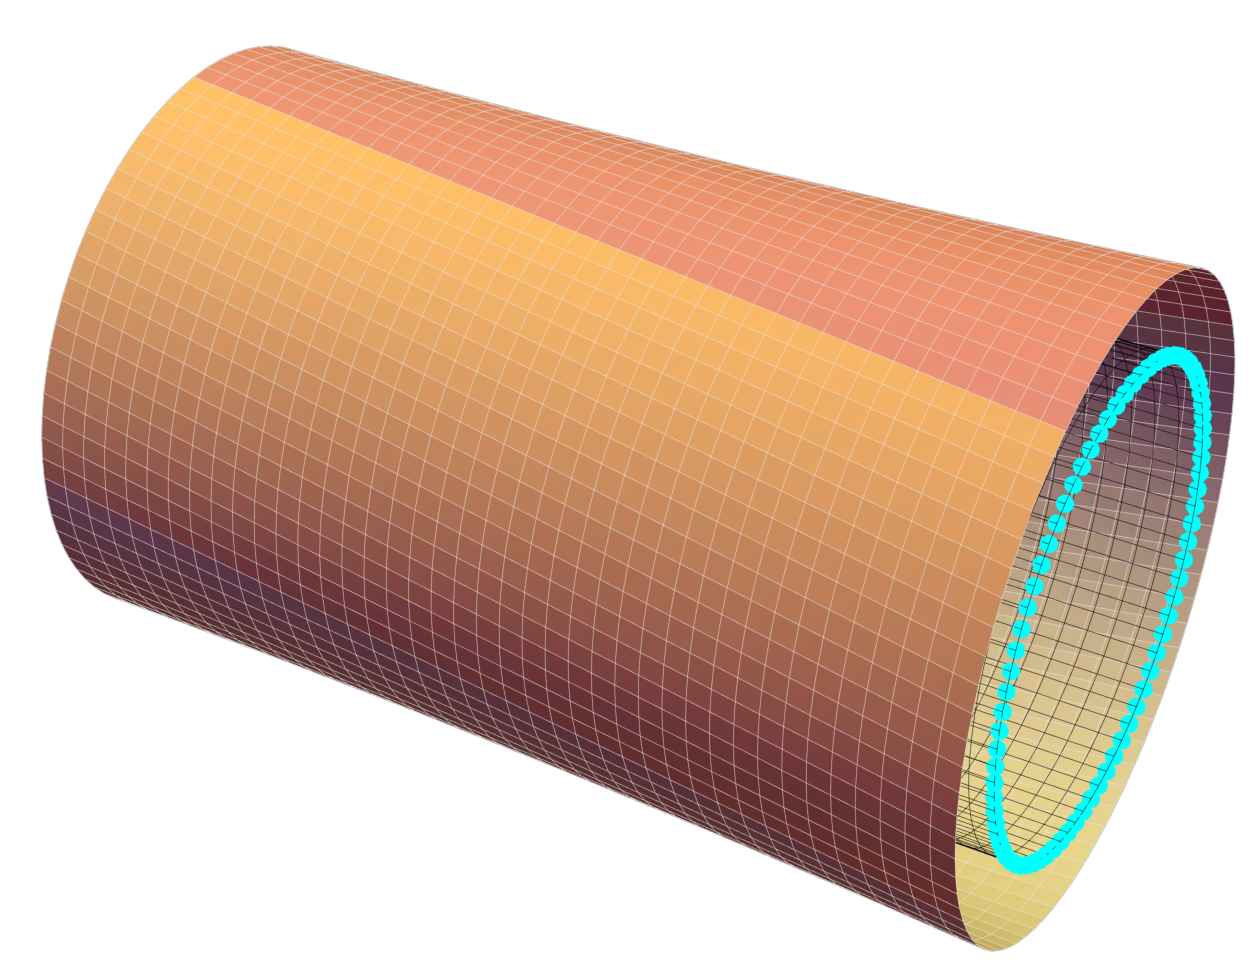
\includegraphics[width=\textwidth]{/more_test/cyl_30_45_30_45.pdf}
	\caption{Elemento tipo cilindro deformato (caso \cref{sec:cyl_D})}
	\label{fig:five ove x}
\end{subfigure}
	\hfill
	\caption{Elementi strutturali}
	\label{fig:three graphs}
\end{figure*}

Per l'analisi della risposta strutturale vengono considerati differenti tipologie di carico. Per l'elemento tipo piasta viene considerato o un carico assiale, o un carico trasversale o entrambi. Per l'elemento tipo cilindro viene invece considerata una pressione interna uniforme.

\subsection{Elemento tipo piastra}

Per l'elemento tipo piastra vengono analizzati i quattro differenti layout di laminato.

\subsubsection{Caso (a)}
\label{sec:plate_A}

\begin{figure*}[bt!]
	\centering

	\begin{subfigure}[t]{0.3\textwidth}
		\centering
		  \scalebox{.5}{
  \def\svgwidth{2\linewidth}
    \input{first_test_bothload_V_X.pdf_tex}}
		\caption{Spostamento lungo $\hat y$ del bordo con $y=0$ della piastra}
		
	\end{subfigure}
	\hfill
	\begin{subfigure}[t]{0.3\textwidth}
		\centering
		  \scalebox{.5}{
	\def\svgwidth{2\linewidth}
	\input{first_test_bothload_W_Y.pdf_tex}}
		
		\caption{Effetto torsionale, spostamento lungo $\hat z$ del bordo estremale della piastra ($x=L$)}
		
	\end{subfigure}
	\hfill
	\begin{subfigure}[t]{0.3\textwidth}
		\centering
		  \scalebox{.5}{
	\def\svgwidth{2\linewidth}
	\input{first_test_bothload_W_X.pdf_tex}}
		\caption{Effetto flessionale, spostamento lungo $z$ del bordo $y=0$ della piastra}
		
	\end{subfigure}
	\hfill
	\caption{Risultati caso (a) per un elemento strutturale tipo piastra con entrambi i carichi (\cref{sec:plate_A})}
	\label{fig:plate_A_both_load}

	\centering
	
	\begin{subfigure}[t]{0.3\textwidth}
		\centering
		  \scalebox{.5}{
	\def\svgwidth{2\linewidth}
	\input{first_test_transload_V_X.pdf_tex}}
		\caption{Spostamento lungo $\hat y$ del bordo con $y=0$ della piastra}
		
	\end{subfigure}
	\hfill
	\begin{subfigure}[t]{0.3\textwidth}
		\centering
		  \scalebox{.5}{
	\def\svgwidth{2\linewidth}
	\input{first_test_transload_W_Y.pdf_tex}}
		
		\caption{Effetto torsionale, spostamento lungo $\hat z$ del bordo estremale della piastra ($x=L$)}
		
	\end{subfigure}
	\hfill
	\begin{subfigure}[t]{0.3\textwidth}
		\centering
		  \scalebox{.5}{
	\def\svgwidth{2\linewidth}
	\input{first_test_transload_W_X.pdf_tex}}
		\caption{Effetto flessionale, spostamento lungo $z$ del bordo $y=0$ della piastra}

	\end{subfigure}
	\hfill
	\caption{Risultati caso (a) per un elemento strutturale tipo piastra con carichi tipo trasversale (\cref{sec:plate_A})}
	\label{fig:plate_A_transload_load}

	\centering
	
	\begin{subfigure}[t]{0.3\textwidth}
		\centering
		  \scalebox{.5}{
	\def\svgwidth{2\linewidth}
	\input{first_test_axialload_V_X.pdf_tex}}
		\caption{Spostamento lungo $\hat y$ del bordo con $y=0$ della piastra}
		
	\end{subfigure}
	\hfill
	\begin{subfigure}[t]{0.3\textwidth}
		\centering
		  \scalebox{.5}{
	\def\svgwidth{2\linewidth}
	\input{first_test_axialload_W_Y.pdf_tex}}
		
		\caption{Effetto torsionale, spostamento lungo $\hat z$ del bordo estremale della piastra ($x=L$)}
		
	\end{subfigure}
	\hfill
	\begin{subfigure}[t]{0.3\textwidth}
		\centering
		  \scalebox{.5}{
	\def\svgwidth{2\linewidth}
	\input{first_test_axialload_W_X.pdf_tex}}
		\caption{Effetto flessionale, spostamento lungo $z$ del bordo $y=0$ della piastra}
				\label{fig:plate_A_extra}
	\end{subfigure}
	\hfill
	\caption{Risultati caso (a) per un elemento strutturale tipo piastra con carichi tipo assiale (\cref{sec:plate_A})}
	\label{fig:plate_A_axial_load}
\end{figure*}



La prima analisi affronta uno studio parametrico (parametro $\alpha$) su un layout del tipo:
\begin{equation}
	\left[\alpha /-\alpha / 30 /-30 / 0_{2}\right]_{\mathrm{S}}
\end{equation}

Vengono considerate tre differenti situazioni di carico: soltanto carico assiale, soltanto carico trasversale ed entrambi i carichi. I risultati sono riportati nelle \cref{fig:plate_A_axial_load,fig:plate_A_transload_load,fig:plate_A_both_load}. 

Al variare del parametro $\alpha$ tra 0° e 90° si osservano risposte strutturali differenti.

Essendo un laminato simmetrico non ci si aspetta un accoppiamento tra gli effetti estensionali e flessionali. Questo viene confermato dal confronto tra i tre casi. È evidente che applicando solo un carico assiale l'effetto flessionale è molto ridotto rispetto le altre configurazioni di carico. Nel caso $\alpha=0^\circ$ la flessione è la minima possibile. Al crescere di $\alpha$ aumenta l'effetto flessionale. Questo non succede con il solo carico assiale dove l'effetto flessionale è molto contenuto e praticamente nullo sia per $\alpha=90^\circ$ che per $\alpha=0^\circ$. In questi ultimi casi è quindi nullo anche l'accoppiamento tra effetti in-plane ed out-plane. 

Ad eccezione dei casi  $\alpha=90^\circ$ e $\alpha=0^\circ$ è sempre presente un effetto torsionale anche se molto contenuto. 

È evidente come la disposizione di un numero maggiore di layer allineati lungo l'asse fornisce meno rigidezza flessionale e questo si rispecchia in un effetto flessionale più marcato. Al fine di ridurre l'effetto flessionale è bene disporre i layer parametrici con  le fibre ortogonali all'asse del laminato. Questo annulla anche l'effetto torsionale e l'accoppiamento in-plane out-plane. Inoltre, fornisce anche maggior rigidezza membranale. Volendo invece avere un effetto flessionale più marcato si possono disporre il maggior numero di layer con le fibre allineate lungo l'asse. Questo porta ad uno spostamento nel lato libero terminale della piastra fino a 5 volte superiore ma rende più evidente l'accoppiamento con gli effetti torsionali. 

È interessante vedere che con il solo carico trasversale, a seconda della configurazione del laminato, è possibile avere una flessione tale da spostare l'estremo finale sia verso l'alto che verso il basso (\cref{fig:plate_A_extra}). Questo effetto non è presente nei casi $\alpha=0^\circ$ o $\alpha=90^\circ$.

I casi intermedi forniscono comportamenti strutturali intermedi tra i due casi limite descritti. L'accoppiameto tra il carico assiale e l'effetto torsionale è massimo per i layout con   $\alpha=20^\circ$ e $\alpha=10^\circ$. 



\subsubsection{Caso (b)}
\label{sec:plate_B}
Viene analizzato un laminato bilanciato con layout:
\begin{equation}
\left[-45 / 45 /-45 / 45\right]
\end{equation}

Nuovamente vengono considerate le tre differenti configurazioni di carico. 

Essendo un laminato bilanciato non ci si aspetta un accoppiamento taglio-estensione. Dai risultati ottenuti, \cref{fig:plate_BD_axial_load,fig:plate_BD_both_load,fig:plate_BD_transload_load}, si osservano diversi accoppiamenti. Si osserva un accoppiamento tra il carico assiale e un effetto flessionale. Si osserva anche un accoppiamento tra il carico assiale e l'effetto torsionale mentre non si osserva un effetto torsionale con il solo carico trasversale. 

Il comportamento di questo laminato è molto simile al comportamento del caso (\cref{sec:plate_A}) con il parametro $\alpha=90^\circ$ ma con una rigidezza flessionale molto minore a causa del minor numero di strati. 


\subsubsection{Caso (c)}
\label{sec:plate_C}

\begin{figure*}[bt!]
	\centering
	
	\begin{subfigure}[t]{0.3\textwidth}
		\centering
		  \scalebox{.5}{
	\def\svgwidth{2\linewidth}
	\input{fabric_bothload_V_X.pdf_tex}}
		\caption{Spostamento lungo $\hat y$ del bordo con $y=0$ della piastra}
		
	\end{subfigure}
	\hfill
	\begin{subfigure}[t]{0.3\textwidth}
		\centering
		  \scalebox{.5}{
	\def\svgwidth{2\linewidth}
	\input{fabric_bothload_W_Y.pdf_tex}}
		
		\caption{Effetto torsionale, spostamento lungo $\hat z$ del bordo estremale della piastra ($x=L$)}
		
	\end{subfigure}
	\hfill
	\begin{subfigure}[t]{0.3\textwidth}
		\centering
		  \scalebox{.5}{
	\def\svgwidth{2\linewidth}
	\input{fabric_bothload_W_X.pdf_tex}}
		\caption{Effetto flessionale, spostamento lungo $z$ del bordo $y=0$ della piastra}
		
	\end{subfigure}
	\hfill
	\caption{Risultati caso (c) per un elemento strutturale tipo piastra con entrambi i carichi (\cref{sec:plate_C})}
	\label{fig:plate_C_both_load}
	\centering
	
	\begin{subfigure}[t]{0.3\textwidth}
		\centering
	  \scalebox{.5}{
	\def\svgwidth{2\linewidth}
	\input{fabric_transload_V_X.pdf_tex}}
		\caption{Spostamento lungo $\hat y$ del bordo con $y=0$ della piastra}
		
	\end{subfigure}
	\hfill
	\begin{subfigure}[t]{0.3\textwidth}
		\centering
	  \scalebox{.5}{
	\def\svgwidth{2\linewidth}
	\input{fabric_transload_W_Y.pdf_tex}}
		
		\caption{Effetto torsionale, spostamento lungo $\hat z$ del bordo estremale della piastra ($x=L$)}
		
	\end{subfigure}
	\hfill
	\begin{subfigure}[t]{0.3\textwidth}
		\centering
	  \scalebox{.5}{
	\def\svgwidth{2\linewidth}
	\input{fabric_transload_W_X.pdf_tex}}
		\caption{Effetto flessionale, spostamento lungo $z$ del bordo $y=0$ della piastra}
		
	\end{subfigure}
	\hfill
	\caption{Risultati caso (c) per un elemento strutturale tipo piastra con carichi tipo trasversale (\cref{sec:plate_C})}
	\label{fig:plate_C_transload_load}

	\centering
	
	\begin{subfigure}[t]{0.3\textwidth}
		\centering
	  \scalebox{.5}{
	\def\svgwidth{2\linewidth}
	\input{fabric_axialload_V_X.pdf_tex}}
		\caption{Spostamento lungo $\hat y$ del bordo con $y=0$ della piastra}
		
	\end{subfigure}
	\hfill
	\begin{subfigure}[t]{0.3\textwidth}
		\centering
	  \scalebox{.5}{
	\def\svgwidth{2\linewidth}
	\input{fabric_axialload_W_Y.pdf_tex}}
		
		\caption{Effetto torsionale, spostamento lungo $\hat z$ del bordo estremale della piastra ($x=L$)}
		
	\end{subfigure}
	\hfill
	\begin{subfigure}[t]{0.3\textwidth}
		\centering
	  \scalebox{.5}{
	\def\svgwidth{2\linewidth}
	\input{fabric_axialload_W_X.pdf_tex}}
		\caption{Effetto flessionale, spostamento lungo $z$ del bordo $y=0$ della piastra}
		
	\end{subfigure}
	\hfill
	\caption{Risultati caso (c) per un elemento strutturale tipo piastra con carichi tipo assiale (\cref{sec:plate_C})}
	\label{fig:plate_C_axial_load}
\end{figure*}

Viene analizzato un layout:
\begin{equation}
\left[\pm 45^{f} / \pm 45^{f}\right]
\end{equation}

Il singolo layer è costituito da uno strato intrecciato, ovvero una configurazione particolare dove le fibre vengono incrociate con direzione di $\pm 45^\circ$. Nel caso di tessuti intrecciati cambia la definizione delle matrice di rigidezza del layer:
\begin{equation}
Q_{i j}^{\text {woven }}=\frac{1}{2}\left[\left(\bar{Q}_{i j}\right)_{45}+\left(\bar{Q}_{i j}\right)_{-45}\right]
\end{equation}

In questo layout non è presente alcun effetto torsionale. 
È assente anche l'accoppiamento tra carichi assiali ed effetto flessionale. 
Il laminato risponde senza mostrare accoppiamenti torsionali o estensionali-flessionali anche a causa della simmetria e del bilanciamento.
 


\subsubsection{Caso (d)}
\label{sec:plate_D}
\begin{figure*}[bt!]
	\centering
	
	\begin{subfigure}[t]{0.3\textwidth}
		\centering
		  \scalebox{.5}{
	\def\svgwidth{2\linewidth}
	\input{BD_bothload_V_X.pdf_tex}}
		\caption{Spostamento lungo $\hat y$ del bordo con $y=0$ della piastra}
		
	\end{subfigure}
	\hfill
	\begin{subfigure}[t]{0.3\textwidth}
		\centering
		  \scalebox{.5}{
	\def\svgwidth{2\linewidth}
	\input{BD_bothload_W_Y.pdf_tex}}
		
		\caption{Effetto torsionale, spostamento lungo $\hat z$ del bordo estremale della piastra ($x=L$)}
		
	\end{subfigure}
	\hfill
	\begin{subfigure}[t]{0.3\textwidth}
		\centering
		  \scalebox{.5}{
	\def\svgwidth{2\linewidth}
	\input{BD_bothload_W_X.pdf_tex}}
		\caption{Effetto flessionale, spostamento lungo $z$ del bordo $y=0$ della piastra}
		\label{fig:plate_BD_extra2}
	\end{subfigure}
	\hfill
	\caption{Risultati caso (b) e (d) per un elemento strutturale tipo piastra con entrambi i carichi (\cref{sec:plate_B,sec:plate_D})}
	\label{fig:plate_BD_both_load}

	\centering
	
	\begin{subfigure}[t]{0.3\textwidth}
		\centering
		  \scalebox{.5}{
	\def\svgwidth{2\linewidth}
	\input{BD_transload_V_X.pdf_tex}}
		\caption{Spostamento lungo $\hat y$ del bordo con $y=0$ della piastra}
		
	\end{subfigure}
	\hfill
	\begin{subfigure}[t]{0.3\textwidth}
		\centering
		  \scalebox{.5}{
	\def\svgwidth{2\linewidth}
	\input{BD_transload_W_Y.pdf_tex}}
		
		\caption{Effetto torsionale, spostamento lungo $\hat z$ del bordo estremale della piastra ($x=L$)}
		
	\end{subfigure}
	\hfill
	\begin{subfigure}[t]{0.3\textwidth}
		\centering
		  \scalebox{.5}{
	\def\svgwidth{2\linewidth}
	\input{BD_transload_W_X.pdf_tex}}
		\caption{Effetto flessionale, spostamento lungo $z$ del bordo $y=0$ della piastra}
		
	\end{subfigure}
	\hfill
	\caption{Risultati caso (b) e (d) per un elemento strutturale tipo piastra con carichi tipo trasversale (\cref{sec:plate_B,sec:plate_D})}
	\label{fig:plate_BD_transload_load}

	\centering
	
	\begin{subfigure}[t]{0.3\textwidth}
		\centering
		  \scalebox{.5}{
	\def\svgwidth{2\linewidth}
	\input{BD_axialload_V_X.pdf_tex}}
		\caption{Spostamento lungo $\hat y$ del bordo con $y=0$ della piastra}
		
	\end{subfigure}
	\hfill
	\begin{subfigure}[t]{0.3\textwidth}
		\centering
		  \scalebox{.5}{
	\def\svgwidth{2\linewidth}
	\input{BD_axialload_W_Y.pdf_tex}}
		
		\caption{Effetto torsionale, spostamento lungo $\hat z$ del bordo estremale della piastra ($x=L$)}
		
	\end{subfigure}
	\hfill
	\begin{subfigure}[t]{0.3\textwidth}
		\centering
		  \scalebox{.5}{
	\def\svgwidth{2\linewidth}
	\input{BD_axialload_W_X.pdf_tex}}
		\caption{Effetto flessionale, spostamento lungo $z$ del bordo $y=0$ della piastra}
		\label{fig:plate_BD_extra}
	\end{subfigure}
	\hfill
	\caption{Risultati caso (b) e (d) per un elemento strutturale tipo piastra con carichi tipo assiale (\cref{sec:plate_B,sec:plate_D})}
	\label{fig:plate_BD_axial_load}
\end{figure*}

Viene analizzato il layout:
\begin{equation}
\left[-30 /-45 /-30 /-45\right]
\end{equation}

I risultati numerici sono presentati nelle \cref{fig:plate_BD_axial_load,fig:plate_BD_both_load,fig:plate_BD_transload_load} confrontati con il caso \cref{sec:plate_B}.  

Questo layout è completamente sbilanciato e asimmetrico con la direzione di fibratura che mostra angoli negativi rispetto l'asse del laminato. Questo si riflette nell'accoppiamento dell'effetto torsionale con tutte le condizioni di carico. 

È presente anche l'accoppiamento in-plane out-plane come è possibile osservare dalla flessione indotta dal solo carico assiale (\cref{fig:plate_BD_extra}).  È molto marcato anche l'accoppiamento estensionale-estensionale. 

È interessante vedere l'effetto del solo carico trasversale (\cref{fig:plate_BD_transload_load}) in cui, a causa dello sbilanciamento delle direzioni di fibratura e della torsione, si ha un effetto complessivo per cui l'estremo libero della piastra tende ad avere uno spostamento in direzione opposta a quella del carico.  Queste effetto, nel caso in cui ci siano entrambe le condizioni di carico, si traduce in un iniziale innalzamento per poi flettersi secondo la direzione del carico trasversale (\cref{fig:plate_BD_extra2}). È riportata anche la deformata completa in \cref{fig:deformata_D}.

Questo accoppiamento si traduce in un effetto flessionale applicando il solo carico longitudinale (\cref{fig:plate_BD_extra}).

\begin{figure}[bt!]
			  \scalebox{.5}{
		\def\svgwidth{2\linewidth}
		\input{deformata_D_tex.pdf_tex}}
	\caption{Deformata nel caso (d) con entrambe le condizioni di carico. La mesh trasparente rappresenta la piastra indeformata. In giallo la piastra deformata, si osservi come il punto A  (vedi anche \cref{fig:plate_BD_extra2}) ha subito uno spostamento negativo mentre il punto B uno spostamento positivo.}
	\label{fig:deformata_D}
\end{figure}

\subsection{Elemento tipo cilindro}

Viene poi considerato un elemento strutturale tipo cilindro con raggio $R$ e lunghezza $L$. Viene considerata una configurazione di carico espressa da una pressione interna uniforme sulla parete del cilindro. Vengono nuovamente analizzati i quattro differenti layout di laminato.

I risultati vengono letti sul bordo del cilindro nei quattro segmenti ottenibili a $x=\pm R$ e $y=\pm R$, così da poter capire se l'allargamento è uniforme o meno lungo l'asse e se è presente un'effetto torsionale. 

\subsubsection{Caso (a)}
\label{sec:cyl_A}
\begin{figure*}[bt!]
	\centering
	\begin{subfigure}[t]{0.23\textwidth}
		\centering
		\scalebox{.5}{
			\def\svgwidth{2\linewidth}
			\input{first_test_C_V_X.pdf_tex}}
		\caption{Spostamento lungo $\hat y$ del bordo con $y=R$ del cilindro}
		
	\end{subfigure}
	\hfill
	\begin{subfigure}[t]{0.23\textwidth}
		\centering
		\scalebox{.5}{
			\def\svgwidth{2\linewidth}
			\input{first_test_C_V_X_2.pdf_tex}}
		
		\caption{Spostamento lungo $\hat y$ del bordo con $y=-R$ del cilindro}
		
	\end{subfigure}
	\hfill
	\begin{subfigure}[t]{0.23\textwidth}
		\centering
		\scalebox{.5}{
			\def\svgwidth{2\linewidth}
			\input{first_test_C_W_X.pdf_tex}}
		\caption{Spostamento lungo $\hat z$ del bordo con $z=R$ del cilindro}
	\end{subfigure}
	\hfill
		\begin{subfigure}[t]{0.23\textwidth}
		\centering
		\scalebox{.5}{
			\def\svgwidth{2\linewidth}
			\input{first_test_C_W_X_2.pdf_tex}}
		\caption{Spostamento lungo $\hat z$ del bordo con $z=-R$ del cilindro}
	\end{subfigure}
	\hfill
	\caption{Risultati caso (a)  per un elemento strutturale tipo cilindro (\cref{sec:cyl_A})}
	\label{fig:cyl_A}
	
		\centering
	\begin{subfigure}[t]{0.23\textwidth}
		\centering
		\scalebox{.5}{
			\def\svgwidth{2\linewidth}
			\input{BD_C_V_X.pdf_tex}}
		\caption{Spostamento lungo $\hat y$ del bordo con $y=R$ del cilindro}
		
	\end{subfigure}
	\hfill
	\begin{subfigure}[t]{0.23\textwidth}
		\centering
		\scalebox{.5}{
			\def\svgwidth{2\linewidth}
			\input{BD_C_V_X_2.pdf_tex}}
		
		\caption{Spostamento lungo $\hat y$ del bordo con $y=-R$ del cilindro}
		
	\end{subfigure}
	\hfill
	\begin{subfigure}[t]{0.23\textwidth}
		\centering
		\scalebox{.5}{
			\def\svgwidth{2\linewidth}
			\input{BD_C_W_X.pdf_tex}}
		\caption{Spostamento lungo $\hat z$ del bordo con $z=R$ del cilindro}
	\end{subfigure}
	\hfill
	\begin{subfigure}[t]{0.23\textwidth}
		\centering
		\scalebox{.5}{
			\def\svgwidth{2\linewidth}
			\input{BD_C_W_X_2.pdf_tex}}
		\caption{Spostamento lungo $\hat z$ del bordo con $z=-R$ del cilindro}
	\end{subfigure}
	\hfill
	\caption{Risultati caso (b) e (d) per un elemento strutturale tipo cilindro (\cref{sec:cyl_B})}
	\label{fig:cyl_BD}
	
			\centering
	\begin{subfigure}[t]{0.23\textwidth}
		\centering
		\scalebox{.5}{
			\def\svgwidth{2\linewidth}
			\input{C_C_V_X.pdf_tex}}
		\caption{Spostamento lungo $\hat y$ del bordo con $y=R$ del cilindro}
		
	\end{subfigure}
	\hfill
	\begin{subfigure}[t]{0.23\textwidth}
		\centering
		\scalebox{.5}{
			\def\svgwidth{2\linewidth}
			\input{C_C_V_X_2.pdf_tex}}
		
		\caption{Spostamento lungo $\hat y$ del bordo con $y=-R$ del cilindro}
		
	\end{subfigure}
	\hfill
	\begin{subfigure}[t]{0.23\textwidth}
		\centering
		\scalebox{.5}{
			\def\svgwidth{2\linewidth}
			\input{C_C_W_X.pdf_tex}}
		\caption{Spostamento lungo $\hat z$ del bordo con $z=R$ del cilindro}
	\end{subfigure}
	\hfill
	\begin{subfigure}[t]{0.23\textwidth}
		\centering
		\scalebox{.5}{
			\def\svgwidth{2\linewidth}
			\input{C_C_W_X_2.pdf_tex}}
		\caption{Spostamento lungo $\hat z$ del bordo con $z=-R$ del cilindro}
	\end{subfigure}
	\hfill
	\caption{Risultati caso (c) per un elemento strutturale tipo cilindro (\cref{sec:cyl_C})}
	\label{fig:cyl_C}
	
\end{figure*}

Viene eseguita una campagna di simulazioni parametrica e analizzata la risposta strutturale al variare del parametro $\alpha$. I risultati sono riportati in \cref{fig:cyl_A}.

Il layout del laminato è del tipo:
\begin{equation}
	\left[\alpha /-\alpha / 30 /-30 / 0_{2}\right]_{\mathrm{S}} \quad \text{ con } \alpha \in \left[0^\circ;90^\circ\right]
\end{equation}


È evidente come al crescere di $\alpha$ i cilindro diventa sempre meno compliante, ovvero a parità di carico si dilata sempre meno. La dilatazione è uniforme e simmetrica, sia lungo $\hat y$ che lungo $\hat z$.

Il maggior numero di fibre orientate parallelamente alla direzione di carico ($\alpha \to 90^\circ$) rende il materiale più rigido e quindi riduce l'effetto estensionale. 

Inoltre, essendo un layout simmetrico e bilanciato, non si osservano neanche effetti di torsione.

\subsubsection{Caso (b)}
\label{sec:cyl_B}

Viene analizzato un laminato bilanciato con layout:
\begin{equation}
	\left[-45 / 45 /-45 / 45\right]
\end{equation}

In questo layout si osserva una dilatazione del cilindro uniforme e simmetrica. La sezione circolare si allarga mantenendosi costante per tutta la lunghezza del cilindro. 

Inoltre, non sono presenti effetti torsionali. 

I risultati sono riportati in \cref{fig:cyl_BD}

\subsubsection{Caso (c)}
\label{sec:cyl_C}
Viene analizzato un layout:
\begin{equation}
	\left[\pm 45^{f} / \pm 45^{f}\right]
\end{equation}

I risultati sono riportati in \cref{fig:cyl_C}.

Il layout intrecciato fornisce complessivamente un layout simmetrico e bilanciato. 

Si osserva una dilatazione uniforme e costante come nei casi precedenti. Numericamente si ottiene una leggera differenza andando a misurare lo spostamento verticale (lungo $\hat z$) del bordo superiore e inferiore, ma è trascurabile e inferiore a $10^{-5}$. Si osserva anche una rigidezza inferiore al caso \cref{sec:cyl_B} a causa anche del minor numero di strati complessivi. 

\subsubsection{Caso (d)}
\label{sec:cyl_D}

Viene analizzato il layout:
\begin{equation}
	\left[-30 /-45 /-30 /-45\right]
\end{equation}

I risultati sono riportati in \cref{fig:cyl_BD} e una deformata tridimensionale è riportata in \cref{fig:five ove x}

Il layout è fortemente sbilanciato e sebbene la dilatazione risulti uniforme si osserva un effetto torsionale. Complessivamente il cilindro tende ad avvitarsi. Questo è possibile osservarlo andando a leggere lo spostamento orizzontale (lungo $\hat y$) del bordo inferiore e superiore del cilindro ($z=\pm R$). Come riportato in \cref{fig:D_extra} si osserva uno spostamento lineare crescente lungo l'asse del cilindro. Risulta positivo per il bordo inferiore e negativo per il bordo superiore.



\begin{figure}[bt!]
	\def\svgwidth{\linewidth}
	\input{D_extra_tex.pdf_tex}
	\caption{Spostamento lungo $\hat y$ per l'elemento strutturale cilindrico nel layout (d) prendendo il bordo a $z=\pm R$. L'anti simmetria presente rispecchia, insieme alle altre considerazioni (vedi \cref{sec:cyl_D} e \cref{fig:five ove x}), la presenza di un effetto torsionale.}
\label{fig:D_extra}
\end{figure}




\section{Spessore della piastra}
\label{sec:final_thick}




\begin{figure*}[bt!]
	\centering
	\begin{subfigure}[c]{0.28\textwidth}
		\centering
		\def\svgwidth{\linewidth}
	\input{struct5_tex.pdf_tex}
		\caption{Layout $\left[10/-10/30/-30/0_2\right]_s$, vedi \cref{sec:final_thick}}
			\label{fig:last_case_schema}
	\end{subfigure}
	\hfill
	\begin{subfigure}[c]{0.28\textwidth}
		\centering
	\def\svgwidth{\linewidth}
		\input{struct5_thickness.pdf_tex}
		\caption{Rappresentazione schematica nello spessore del layout  $\left[10/-10/30/-30/0_2\right]_s$ dove sono presenti 12 strati con uno spessore $t=0.2$ ciascuno.}
		
	\end{subfigure}
	\hfill
	\begin{subfigure}[c]{0.35\textwidth}
		\centering
	\def\svgwidth{\linewidth}
	\input{struct5_thickness_sigmaX_.pdf_tex}
		\caption{Rappresentazione qualitativa dell'andamento lineare a tratti delle tensioni $\sigma_x$ nello spessore della piastra (vedi \cref{sec:final_thick}). Il grafico è stato estratto dalla \cref{fig:sigma_x} ed è stato scalato. }
		
	\end{subfigure}
	\hfill
	\caption{Rappresentazione del layout considerato nella sezione \cref{sec:final_thick} }
	\label{fig:last_case}
\end{figure*}

\begin{figure*}[bt!]
	\centering
	
	\begin{subfigure}[t]{0.3\textwidth}
		\centering
		\scalebox{.5}{
			\def\svgwidth{2\linewidth}
			\input{last_layer_V_X.pdf_tex}}
		\caption{Spostamento lungo $\hat y$ del bordo con $y=0$ della piastra}
		
	\end{subfigure}
	\hfill
	\begin{subfigure}[t]{0.3\textwidth}
		\centering
		\scalebox{.5}{
			\def\svgwidth{2\linewidth}
			\input{last_layer_W_Y.pdf_tex}}
		
		\caption{Effetto torsionale, spostamento lungo $\hat z$ del bordo estremale della piastra ($x=L$)}
		
	\end{subfigure}
	\hfill
	\begin{subfigure}[t]{0.3\textwidth}
		\centering
		\scalebox{.5}{
			\def\svgwidth{2\linewidth}
			\input{last_layer_W_X.pdf_tex}}
		\caption{Effetto flessionale, spostamento lungo $z$ del bordo $y=0$ della piastra}
	\end{subfigure}
	\hfill
	\caption{Rappresentazioni degli spostamenti al variare del moltiplicatore di carico $\lambda \in \left\{1; 2; 5;10;20;30\right\}$}
	\label{fig:last_layer}
	
	\centering
	
	\begin{subfigure}[t]{0.3\textwidth}
		\centering
		\scalebox{.5}{
			\def\svgwidth{2\linewidth}
			\input{grafico_sigma_x.pdf_tex}}
		\caption {Rappresentazione delle tensioni $\sigma_x$}
				\label{fig:sigma_x}
	\end{subfigure}
	\hfill
	\begin{subfigure}[t]{0.3\textwidth}
		\centering
		\scalebox{.5}{
			\def\svgwidth{2\linewidth}
			\input{grafico_sigma_y.pdf_tex}}
		
		\caption{Rappresentazione delle tensioni $\sigma_y$}
		
	\end{subfigure}
	\hfill
	\begin{subfigure}[t]{0.3\textwidth}
		\centering
		\scalebox{.5}{
			\def\svgwidth{2\linewidth}
			\input{grafico_tau_xy.pdf_tex}}
		\caption{Rappresentazione delle tensioni $\tau_{xy}$}
			\label{fig:stress}
	\end{subfigure}
	\hfill
	\caption{Rappresentazioni delle tensioni al variare del moltiplicatore di carico $\lambda \in \left\{1; 2; 5;10;20;30\right\}$}

\end{figure*}


Nella teoria dei laminati sottili il campo di deformazione viene ridotto ad un campo di deformazione della superficie media legato a scorrimenti e dilatazioni nel piano. A questo si aggiungono effetti fuori dal piano legati all'inflessione della superficie media e ad eventuali contributi di torsione. Questo implica che il campo di deformazione viene assunto costante e identico in tutti i layer.

Si considera allora un ulteriore caso con 12 layer aventi un layout del tipo:
\begin{equation}
	[10 /-10 / 30 /-30 / 0_2]_{\mathrm{s}}
\end{equation}

Una rappresentazione schematica è illustrata in \cref{fig:last_case_schema}. 

L'unica cosa che distingue un layer dall'altro, secondo la teoria considerata, è la sola coordinata $z$. Quindi possiamo considerare il legame ridotto nel piano dove ogni layer avrà  il suo aspetto costitutivo mentre le deformazioni saranno legate allla coordinata $z$. 

\begin{equation}
	\begin{bmatrix}
		\sigma_x\\ \sigma_y\\ \tau_{xy}
	\end{bmatrix}_k=
\begin{bmatrix}
	\bar Q
\end{bmatrix}_k \begin{bmatrix} \varepsilon_x\\ \varepsilon_y\\ \gamma_{xy} \end{bmatrix}
\label{eq:QQ}
\end{equation}

Ovvero lo stato di tensione sarà continuo nel layer ma discontinuo all'interfaccia e al più varierà linearmente lungo lo spessore a causa della dipendenza lineare della deformazione \cref{fig:layout}.

Viene applicato un certo carico assiale fisso mentre il carico trasversale scalato tramite un moltiplicatore, \cref{eq:Tload}, così da poter analizzare la variazione delle tensioni interne al variare del carico trasversale. 

\begin{equation}
	\lambda \:F_{\perp} \quad \text{con } \lambda \in \left\{1; 2; 5;10;20;30\right\}
	\label{eq:Tload}
\end{equation}
\begin{figure}[bt!]
	\centering\captionsetup[subfigure]{justification=centering}
	\begin{subfigure}{0.25\linewidth}
		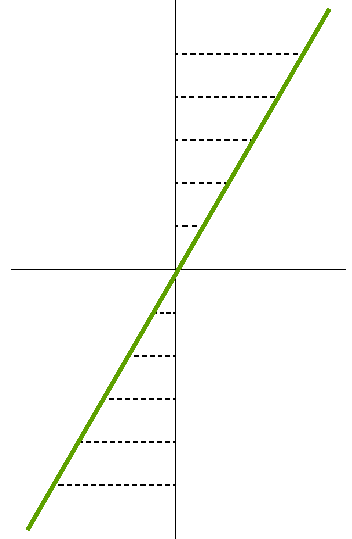
\includegraphics[width=\textwidth]{strain.pdf}
		\caption{}
	\end{subfigure}\hspace{0.1\linewidth}
	\begin{subfigure}{0.25\linewidth}
		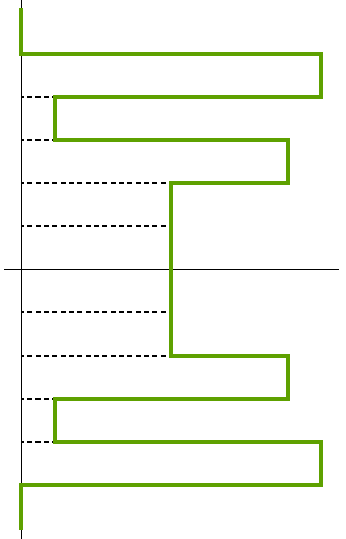
\includegraphics[width=\textwidth]{Q.pdf}
		\caption{}
	\end{subfigure}\hspace{0.1\linewidth}
	\begin{subfigure}{0.25\linewidth}
		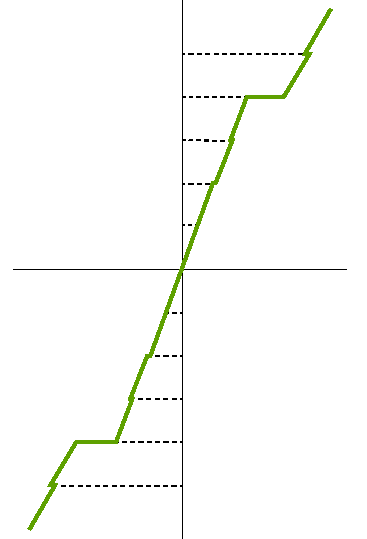
\includegraphics[width=\textwidth]{stress.pdf}
		\caption{}
	\end{subfigure}
	\caption{Rappresentazione grafica dell'\cref{eq:QQ} nello spessore del laminato. Sono rappresentate le deformazioni (i), la rigidezza (ii) e le tensioni (iii). }
	\label{fig:layout}
\end{figure}

È evidente come lo spostamento risulti proporzionale al carico applicato, al crescere del moltiplicatore di carico aumenta la flessione. 

Sono assenti effetti torsionali essendo un laminato simmetrico e bilanciato.

Non sono presenti effetti estensionali e lo spostamento lungo $\hat y$ del bordo della piastra è inferiore a $5 \cdot 10^{-4}$. 

Andando a vedere le tensioni lungo lo spessore, ovvero al varare della coordinata $z \in \left[-{h\over 2};{h\over 2}\right]$ è possibile vedere l'andamento lineare a tratti. L'andamento lineare è dato dalle deformazioni che moltiplicano un coefficiente di rigidezza diverso layer per layer (vedi \cref{fig:layout}). 

Anche le tensioni crescono, in modulo, proporzionalmente al moltiplicatore di carico. 





\section{Conclusioni}

Conoscere la risposta di elementi strutturali può essere utile per modellare correttamente una determinata struttura in laminato composito e per fare studi dettagliati di danno analizzando le tensioni interne.

Alcuni casi possono essere semplici da prevedere come l'allineamento di tutte le fibre lungo una stessa direziond. Casi più complessi, come layout sbilanciati, possono portare a comportamenti strutturali non sempre facili da predire. 

Implementare un'analisi del composito laminato che porta in conto la configurazione dei singoli layer fornisce risultati utili alla comprensione del comportamento strutturale.

Inoltre, permette di tenere in conto anche delle tensioni interne nei singoli layer che presentano una discontinuità all'interfaccia layer-layer. 

\section{Metodi}

\begin{figure*}[b]
	\begin{lstlisting}[language=Mathematica,caption=Struttura del codice per la simulazione nel caso \cref{sec:plate_A},label=code_general]
		<< AceFEM`;
		SimulationComplete[alpha_, axialLoad_, trasLoad_] := (
		displacement = Table[{0*i, 0, 0}, {i, 1, Length[alpha]}];
		Do[ 
		Print["$\alpha$=", alpha[[i]]];
		MyGeometry[alpha[[i]], axialLoad, trasLoad];
		FEMModel[];
		Coordinate[];
		Solution[];
		Print[Show[SMTShowMesh["DeformedMesh" -> True, "Mesh" -> GrayLevel[0.9]], SMTShowMesh["FillElements" -> False, "BoundaryConditions" -> True, "Mesh" -> GrayLevel[0]]]];
		displacement[[i]] = PostProcessMyDisplacement[alpha[[i]]];, 
		{i, 1, Length[alpha]}];
		PrintMyDisplacement[displacement, alpha];   		;
		(***)
		alpha = {0, 10, 20, 30, 40, 50, 60, 70, 80, 90};
		axLoad = 2*10^3* (L/10);
		trLoad = 0.02*10^3;
		SimulationComplete[alpha, axLoad, trLoad]
	\end{lstlisting}
	\begin{lstlisting}[language=Mathematica,caption=Snippet di \texttt{total$\mathbb Q$[]} che si occupa di generare il layout del laminato a partire dalla definizione di ogni layer,label=code_totalq]
index = 0; 
totalLayer = Total[Table[layer[[i, 1]], {i, 1, Length[layer]}]];
$\mathbb Q$$\mathbb Q$ = Table[DiagonalMatrix[{0, 0, 0}]*i, {i, 1, totalLayer}];
$\theta$$\theta$ = Table[DiagonalMatrix[{0, 0, 0}]*i, {i, 1, totalLayer}];
zzv = Table[0*i, {i, 1, totalLayer + 1}];
Do[Do[ $\theta$$\theta$[[index + j]] = layer[[i, 2]];
zzv[[index + j + 1]] = zzv[[index + j]] + layer[[i, 7]];
$\mathbb Q$$\mathbb Q$[[index + j]] = Calc$\mathbb Q$[layer[[i, 3]], layer[[i, 4]], layer[[i, 5]], layer[[i, 6]]], 
{j, 1, layer[[i, 1]]}];  index = index + layer[[i, 1]]; ,   {i, 1, Length[layer]}];
zzv = zzv - (Abs[zzv[[1]] + zzv[[Length[zzv]]]]/2);
Return[{$\mathbb Q$$\mathbb Q$, zzv, $\theta$$\theta$}] 
\end{lstlisting}

\end{figure*}

Per implementare le campagne di simulazione è stato utilizzato il software \texttt{Mathematica} \citep{mathematica} con il pacchetto aggiuntivo\texttt{ AceGEN/AceFEM} \citep{ace}. 


\subsection{Legame costitutivo generalizzato}


Per il calcolo del legame costitutivo generalizzato e quindi le tre matrici $\mathbb A, \mathbb B, \mathbb D$ viene utilizzata la funzione \texttt{ABDcomp1[$\theta v$, $zv$, $\mathbb Q]$} a cui vengono passati:
\begin{itemize}
	\item \texttt{$\theta v$}, vettore contenente l'angolo di ogni layer
	\item \texttt{$zv$}, vettore contenente la coordinata iniziale e finale nello spessore di ogni layer
	\item \texttt{$\mathbb Q$}, matrice di rigidezza del layer ottenuta con la regola delle miscele nel riferimento locale
\end{itemize}

L'algoritmo ruota la matrice di rigidezza nel riferimento globale ( \cref{eq:rotazione}) e poi calcola le tre matrici costitutive, vedi \cref{eq:A,eq:B,eq:D}.



\subsection{Simulazione}

Tutte le diverse campagne di simulazione sono basate sulla stessa logica. Utilizzano alcune routine per separare diverse sezioni implmentative, molte comuni tra i diversi casi analizzati.

La simulazione viene avviata passando alla routine \texttt{SimulationComplete[]} il layout del laminato e il carico. Tale routine (un esempio è presente nello snippet \ref{code_general}) comprende:
\begin{itemize}
	\item \texttt{MyGeometry[]}
	\item \texttt{FEM Model[]}
   \item \texttt{Coordinate[]}
	\item \texttt{Solution[]}
	\item \texttt{PostProcessMyDisplacement[]}
\end{itemize}

Ciascuna sotto routine ha un suo compito preciso. 

La subroutine \texttt{MyGeometry[]} si occupa di richiamare la funzione \texttt{ABDcomp1[]}  passandogli la definizione  del layout e di ogni singolo layer.  Provvede anche ad impostare le dimensioni generali dell'elemento strutturale. Prima di passare i dati alla routine \texttt{ABDcomp1[]} vengono passati a \texttt{total$\mathbb Q$[]} che si occupa di calcolare le coordinate di spessore e preparare un vettore unico sia per l'angolo di rotazione che per la matrice di rigidezza di ogni layer.

 \texttt{FEM Model[]} inizializza il modello agli elementi finiti definendo le proprietà della mesh e le condizioni al bordo.
 
 \texttt{Coordinate[]} si occupa della definizione delle coordinate locali e applica il carico trasversale sulle coordinate nodali di interesse.
 
 La routine  \texttt{Solution[]} provvede alla risoluzione tramite il metodo di Newton Rapson con passi di carico fissi. 
 
 Infine la sotto routine \texttt{PostProcessMyDisplacement[]} si occupa di generare tutti i grafici e di stampare la deformata.
 
Chiaramente la funzione \texttt{SimulationComplete[]} viene inserita all'interno di un ciclo sul parametro di interesse, ad esempio l'angolo $\alpha$ per il caso \cref{sec:plate_A} o il carico per il caso \cref{sec:final_thick}.



\section{Disponibilità del codice e materiale aggiuntivo}

Tutto il codice, le immagini, file di processamento e risultati ottenuti sono disponibili alla repository online al link: \url{https://github.com/mastroalex/comp-lam}

Sono compresi:

\begin{itemize}
	\item Notebook per i casi nelle \cref{sec:plate_A,sec:cyl_A} in \texttt{first\_test->frst\_test\_final.nb}
	\item  Notebook per i casi nelle \cref{sec:plate_B,sec:plate_D,sec:cyl_B,sec:cyl_D} in \texttt{more\_test->more\_test\_final.nb}
	\item  Notebook per i casi nelle \cref{sec:plate_C,sec:cyl_C} in \texttt{more\_test->FABRIC->more\_test\_final\_fabric.nb}
	\item  Notebook per il caso in \cref{sec:final_thick} in \texttt{more\_test->LAST\_LAYER->more\_test\_final\_layer.nb}

\end{itemize}




%% Specify your .bib file name here, without the extension
%\newpage
%\onecolumn

\newpage
\bibliography{paper-refs}




\end{document}
